\documentclass{article}

\usepackage{amsmath}
\usepackage{hyperref}
\usepackage{graphicx}

%%%%%%%%%%%%%%%%%%%%%%%%%%%%%%


\title{Web-based Supplementary Materials for Quantile Regression in the Presence of Monotone Missingness with Sensitivity Analysis by (Minzhao Liu, Michael J. Daniels and Michael G. Perri)}

\begin{document}

\maketitle

\section{Web  Figure 1}

\begin{figure}[h]
\centerline{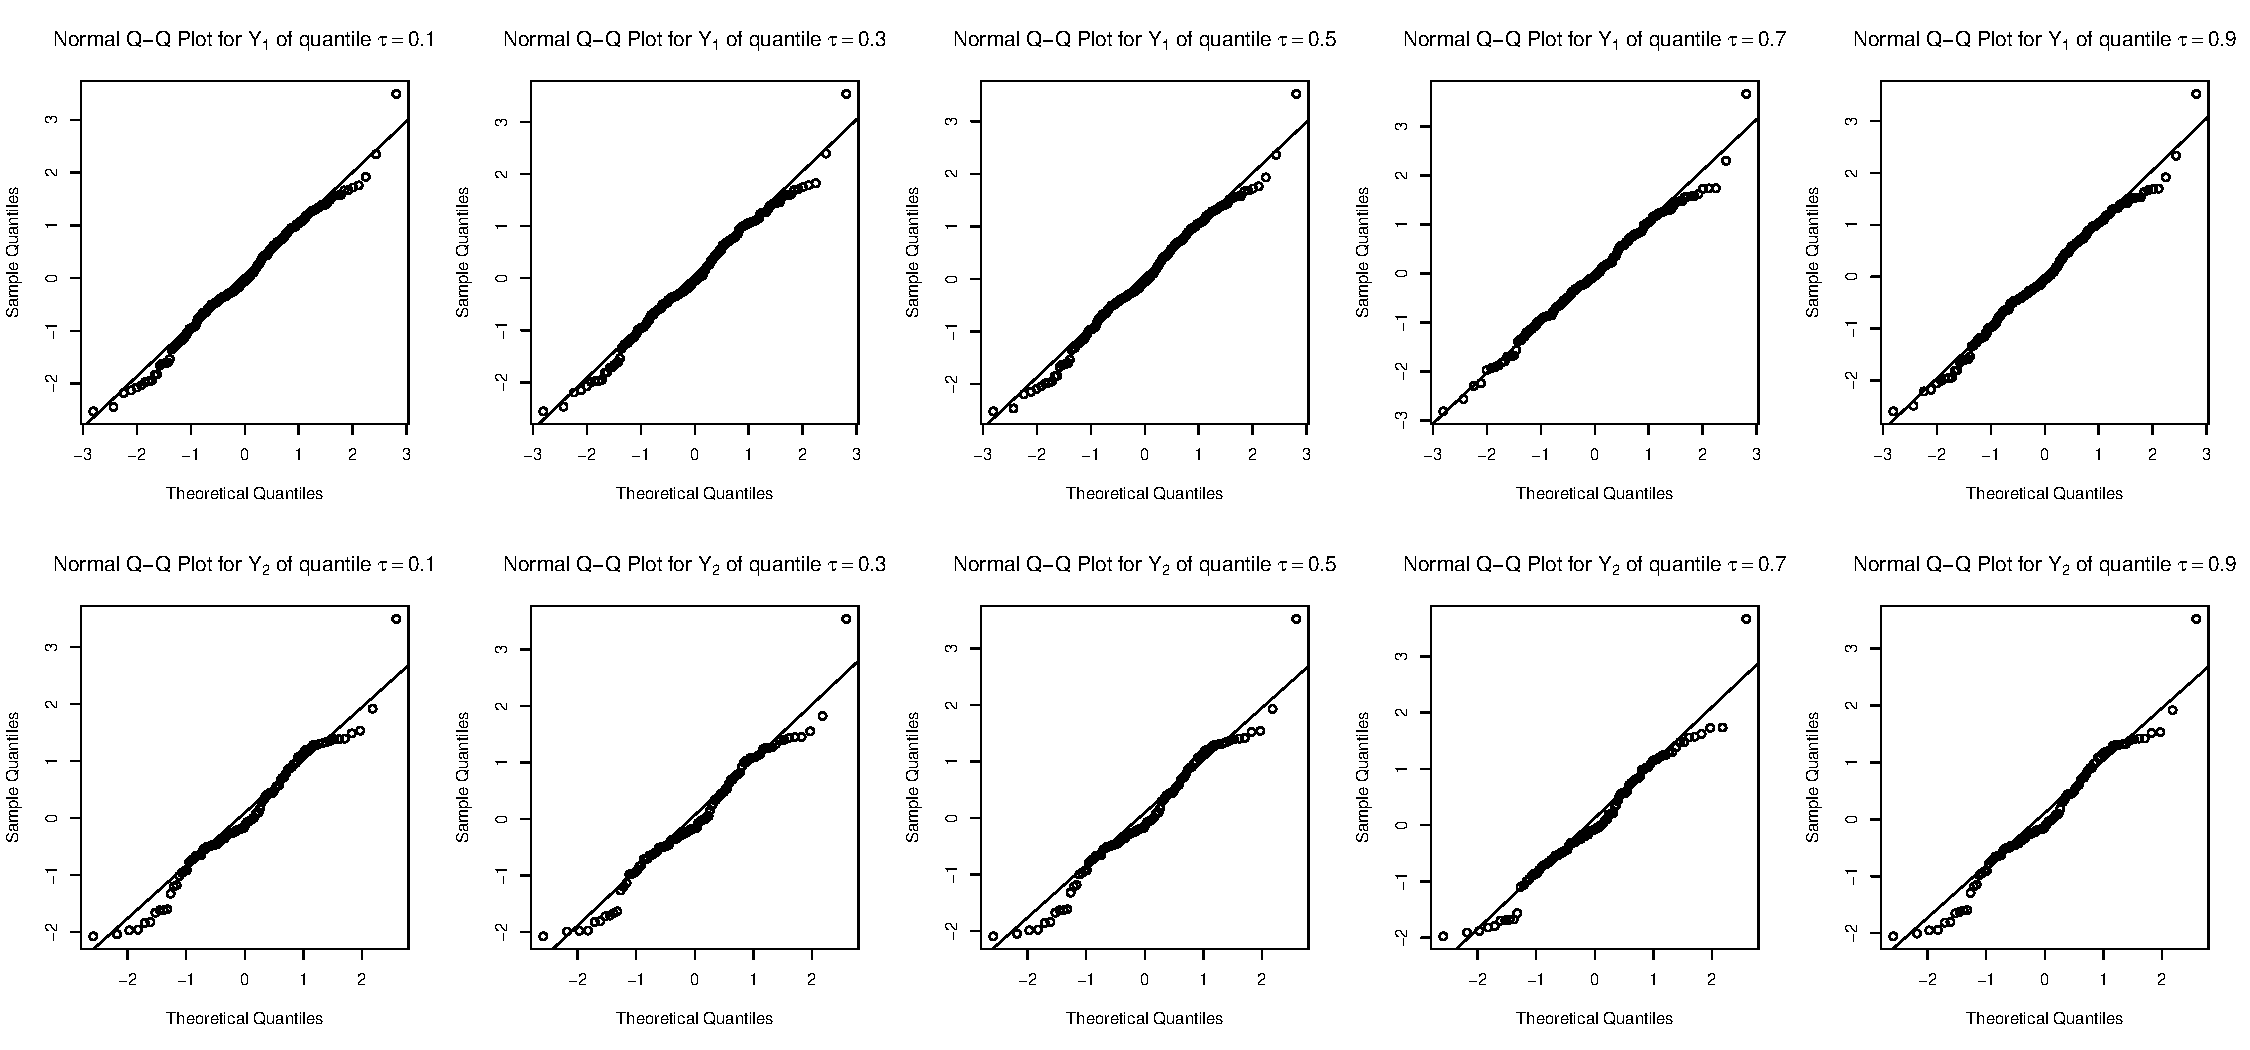
\includegraphics[scale=.4]{../image/NormalS1}}
\caption{Goodness of Fit Check for Normal Error under Scenario 1}
\end{figure}

\begin{figure}[h]
\centerline{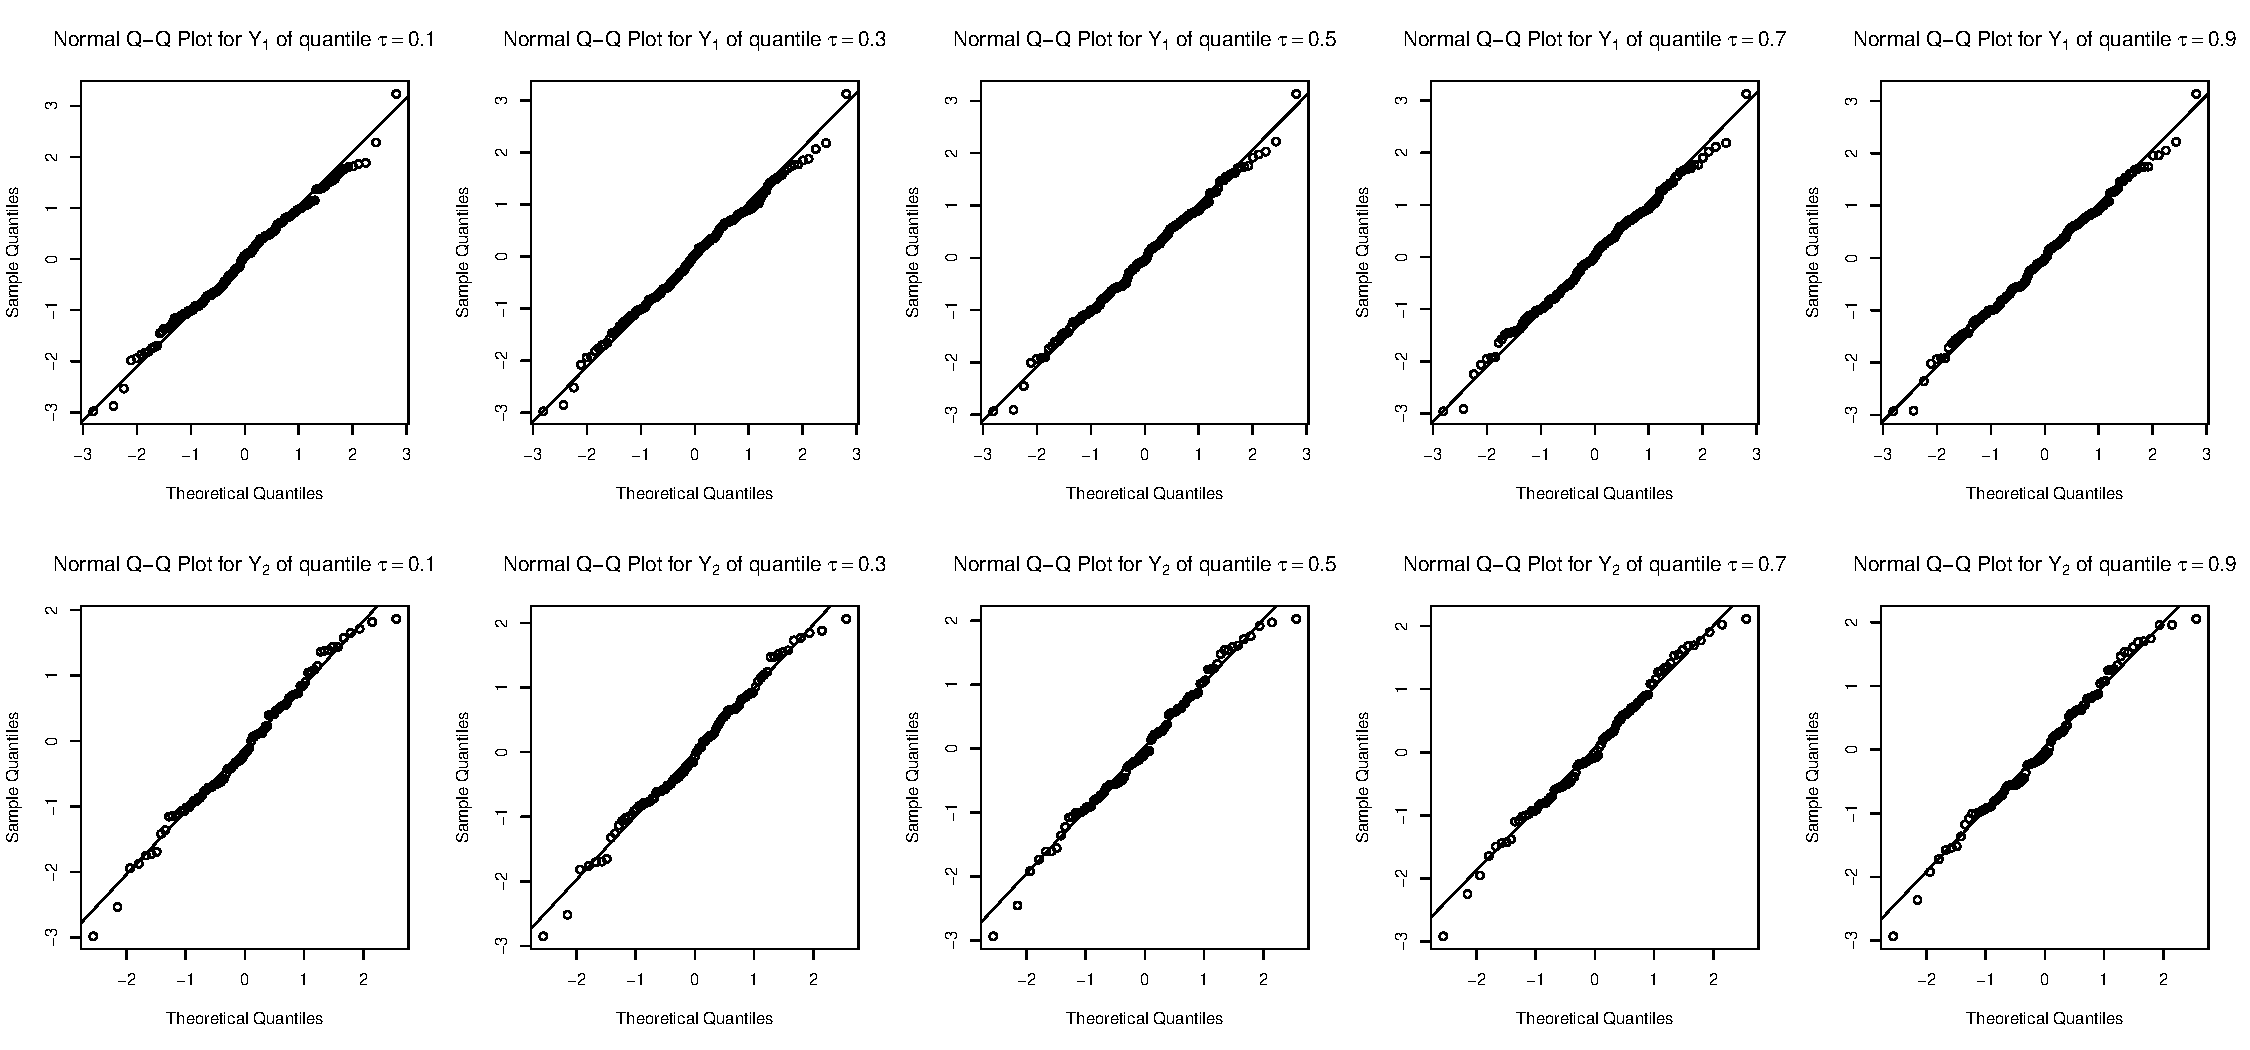
\includegraphics[scale=.4]{../image/NormalS2}}
\caption{Goodness of Fit Check for Normal Error under Scenario 2}
\end{figure}

\begin{figure}[h]
\centerline{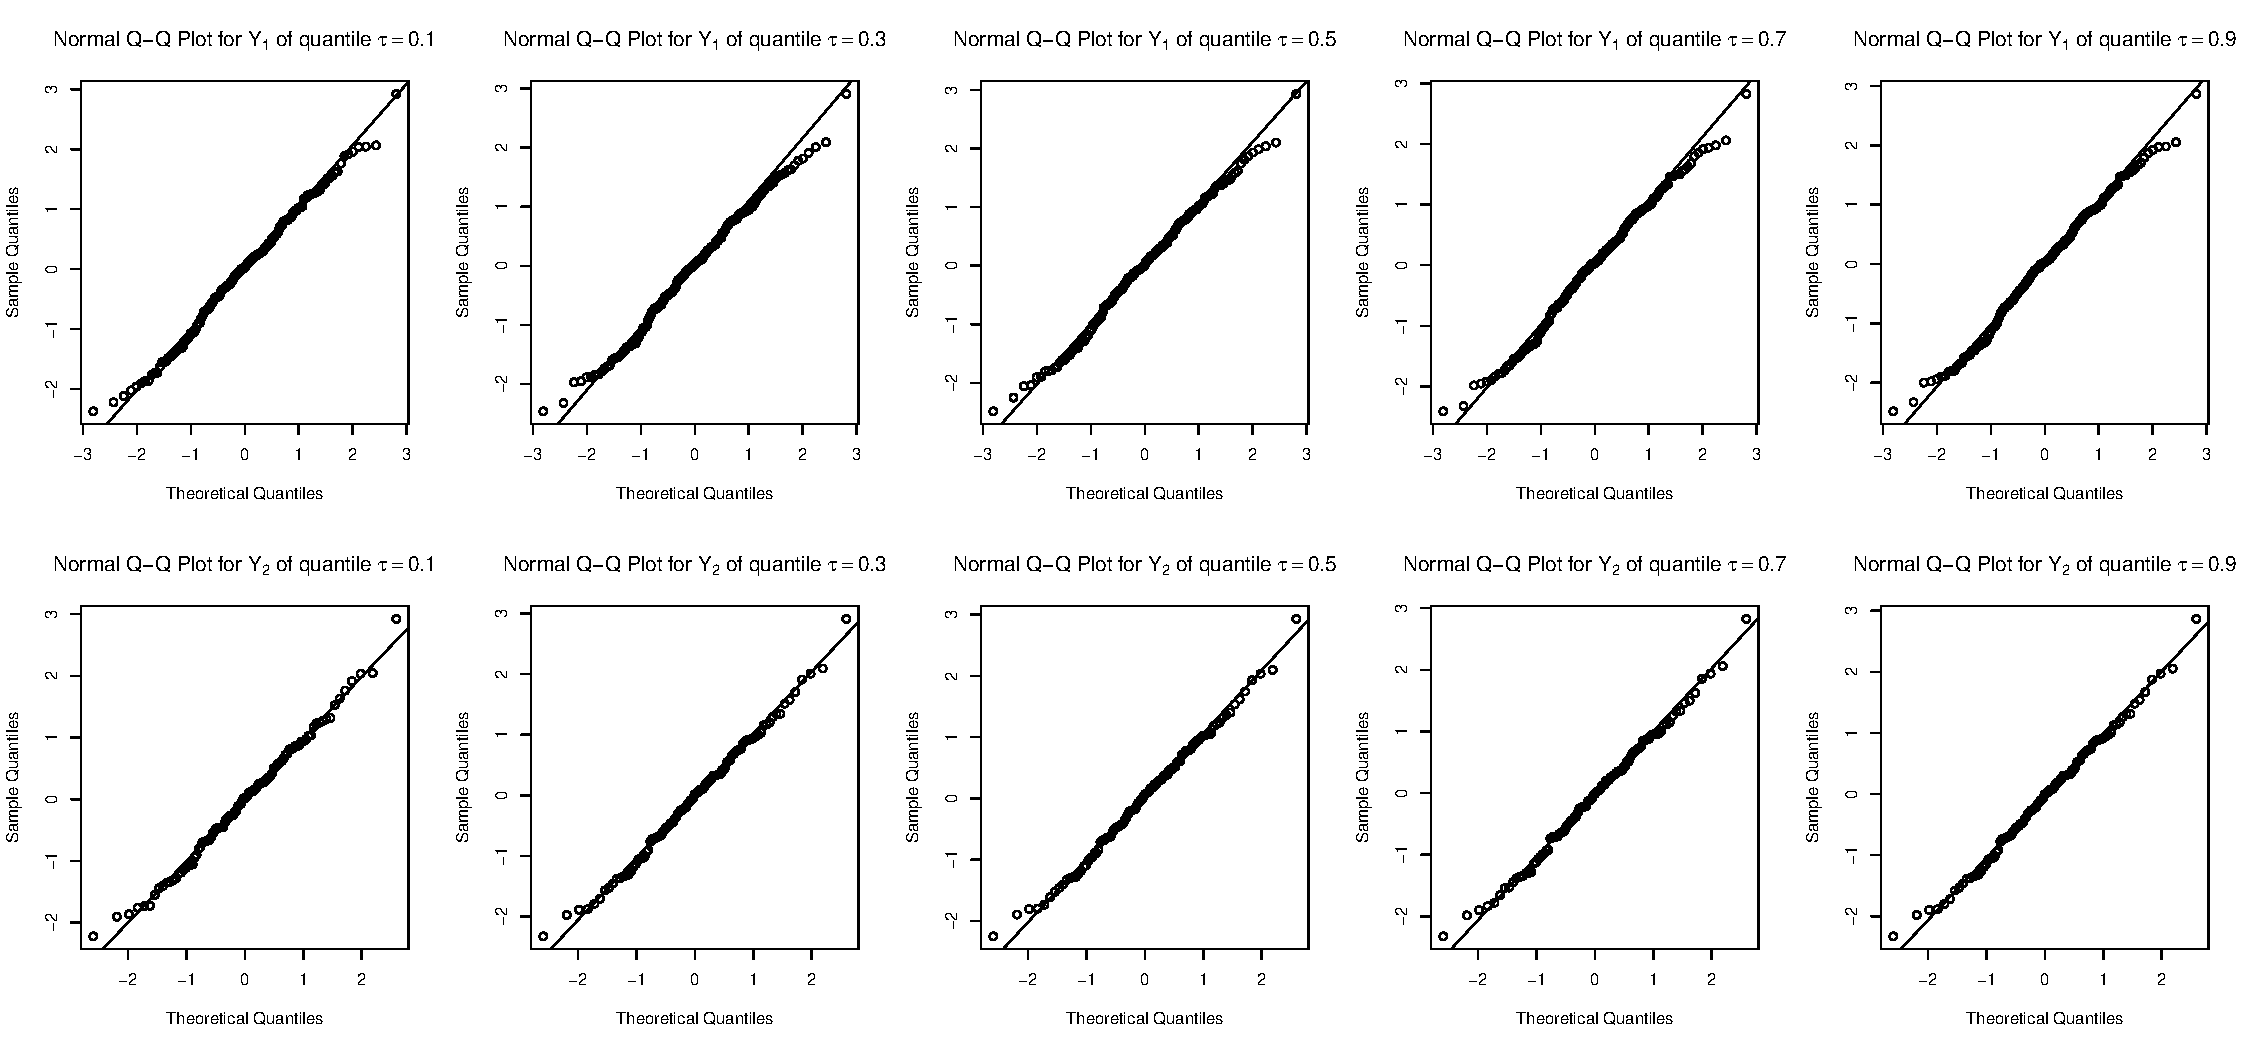
\includegraphics[scale=.4]{../image/NormalS3}}
\caption{Goodness of Fit Check for Normal Error under Scenario 3}
\end{figure}

\begin{figure}[h]
\centerline{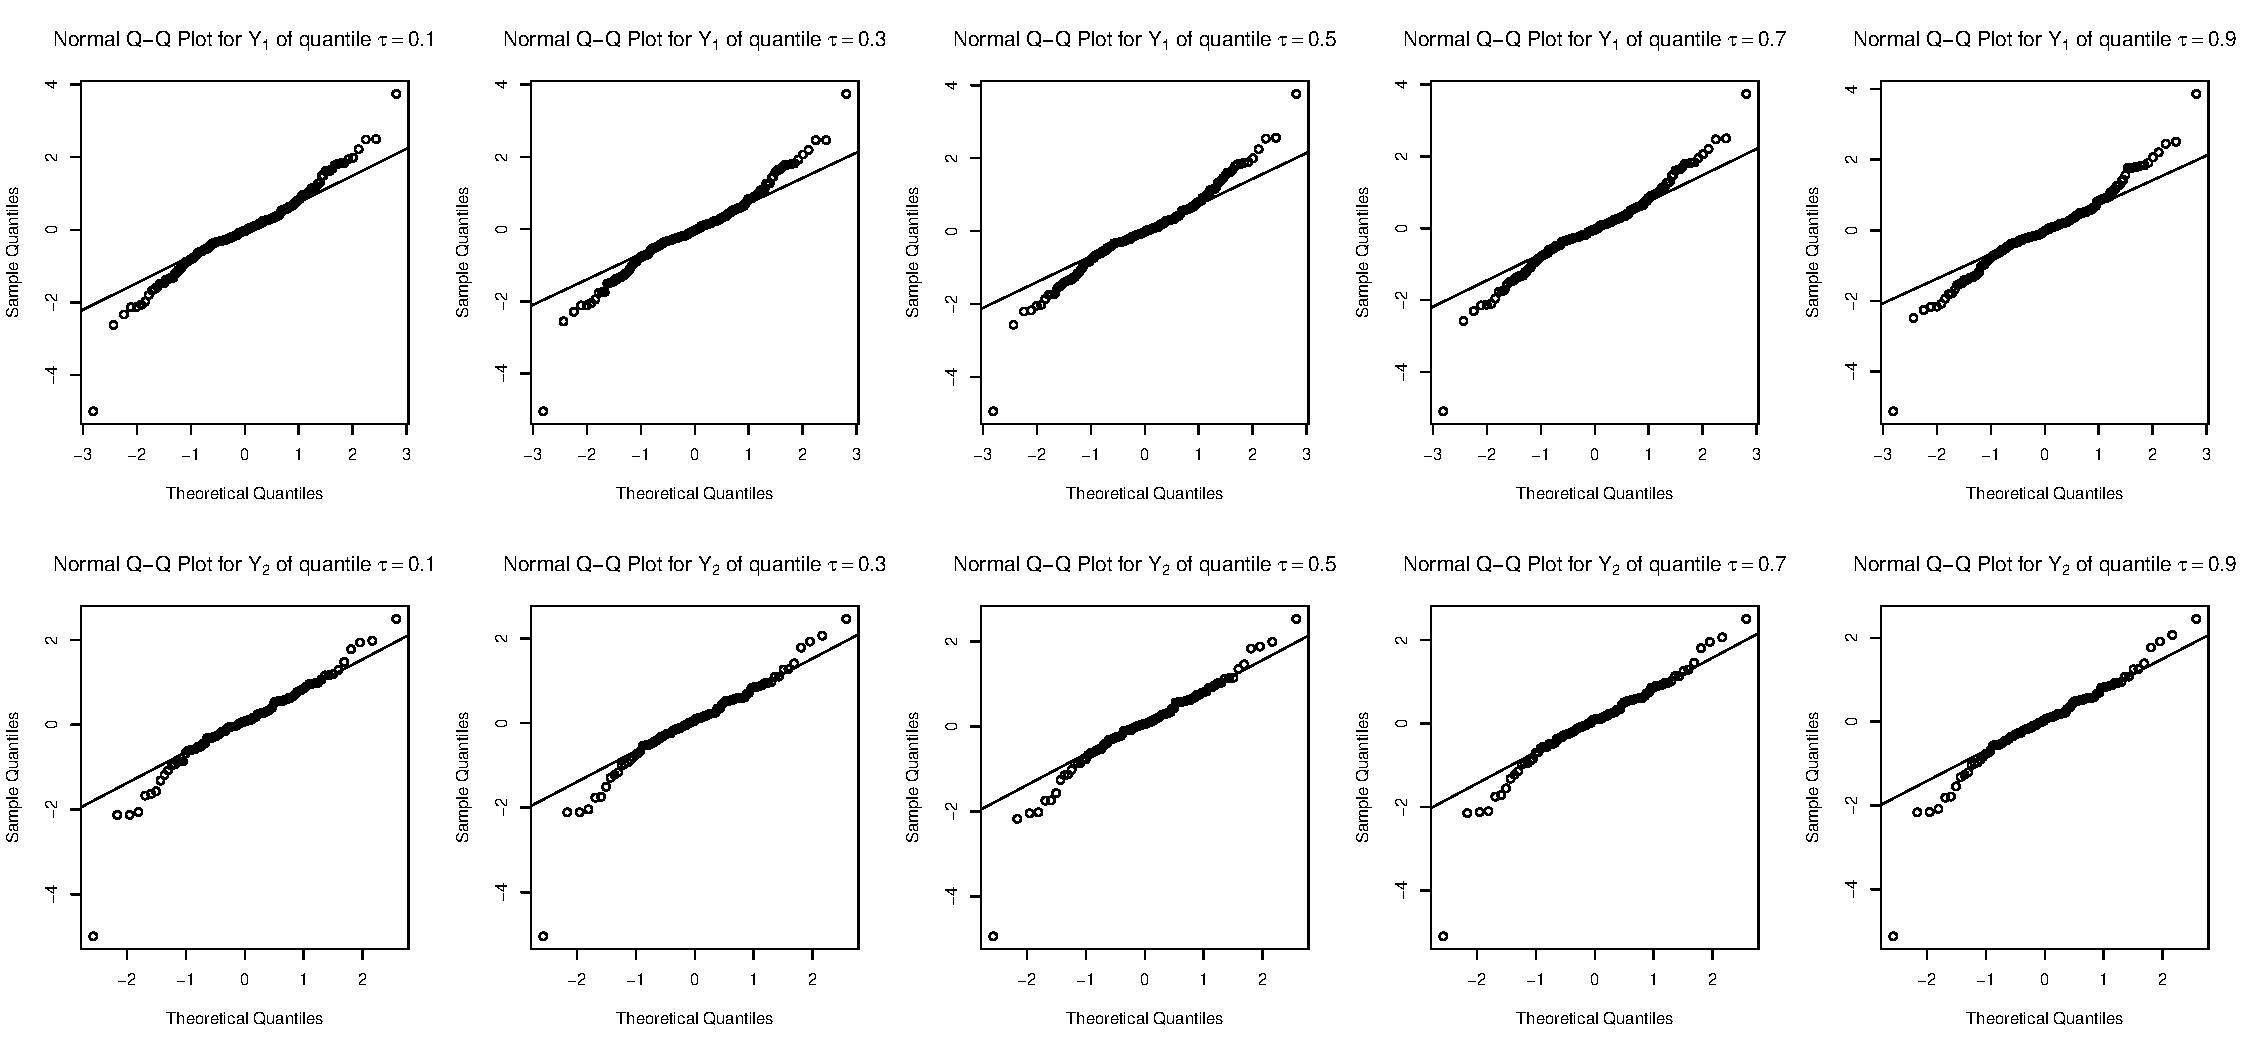
\includegraphics[scale=.4]{../image/T3S1}}
\caption{Goodness of Fit Check for $t_3$ Error under Scenario 1}
\end{figure}

\begin{figure}[h]
\centerline{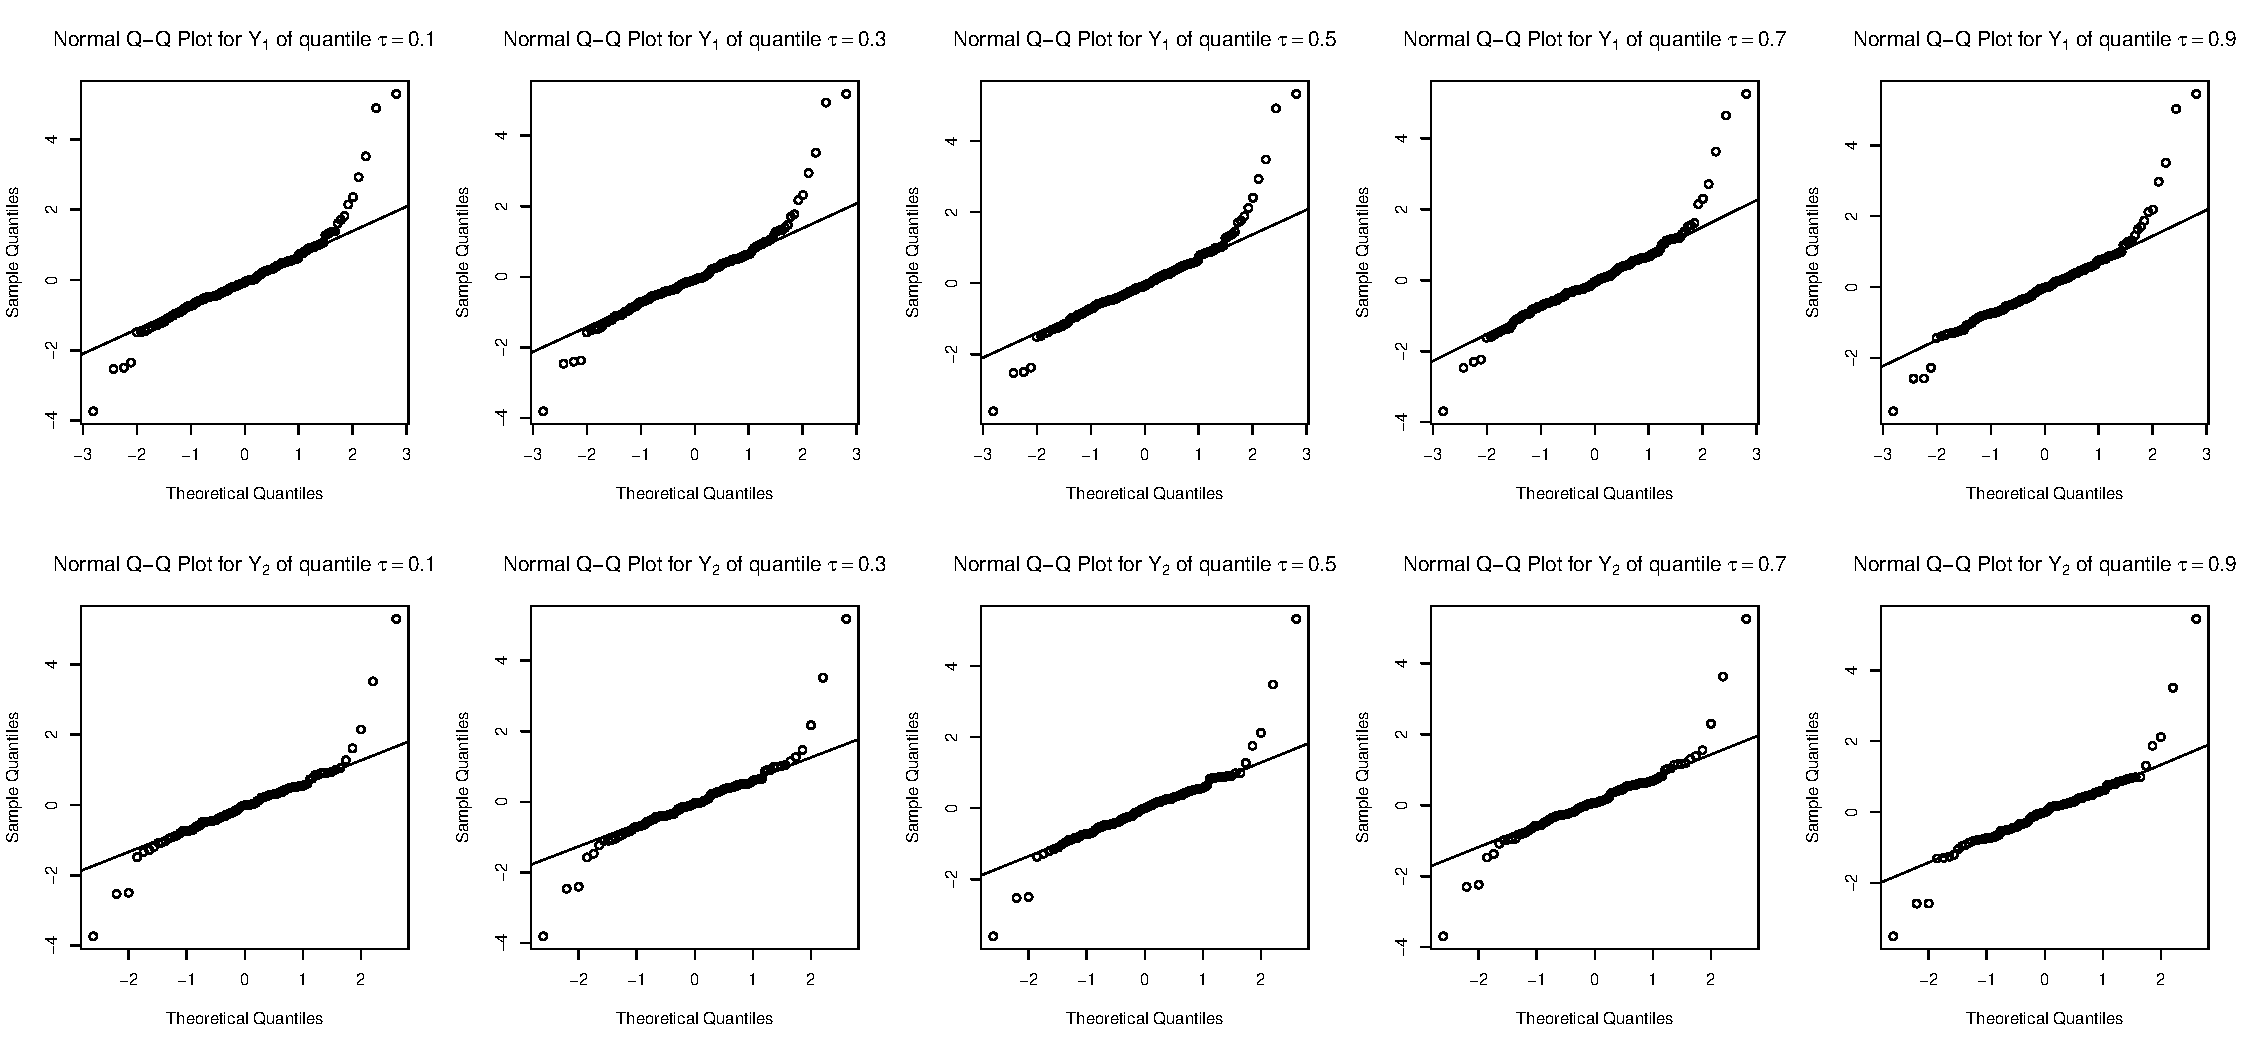
\includegraphics[scale=.4]{../image/T3S2}}
\caption{Goodness of Fit Check for $t_3$ Error under Scenario 2}
\end{figure}

\begin{figure}[h]
\centerline{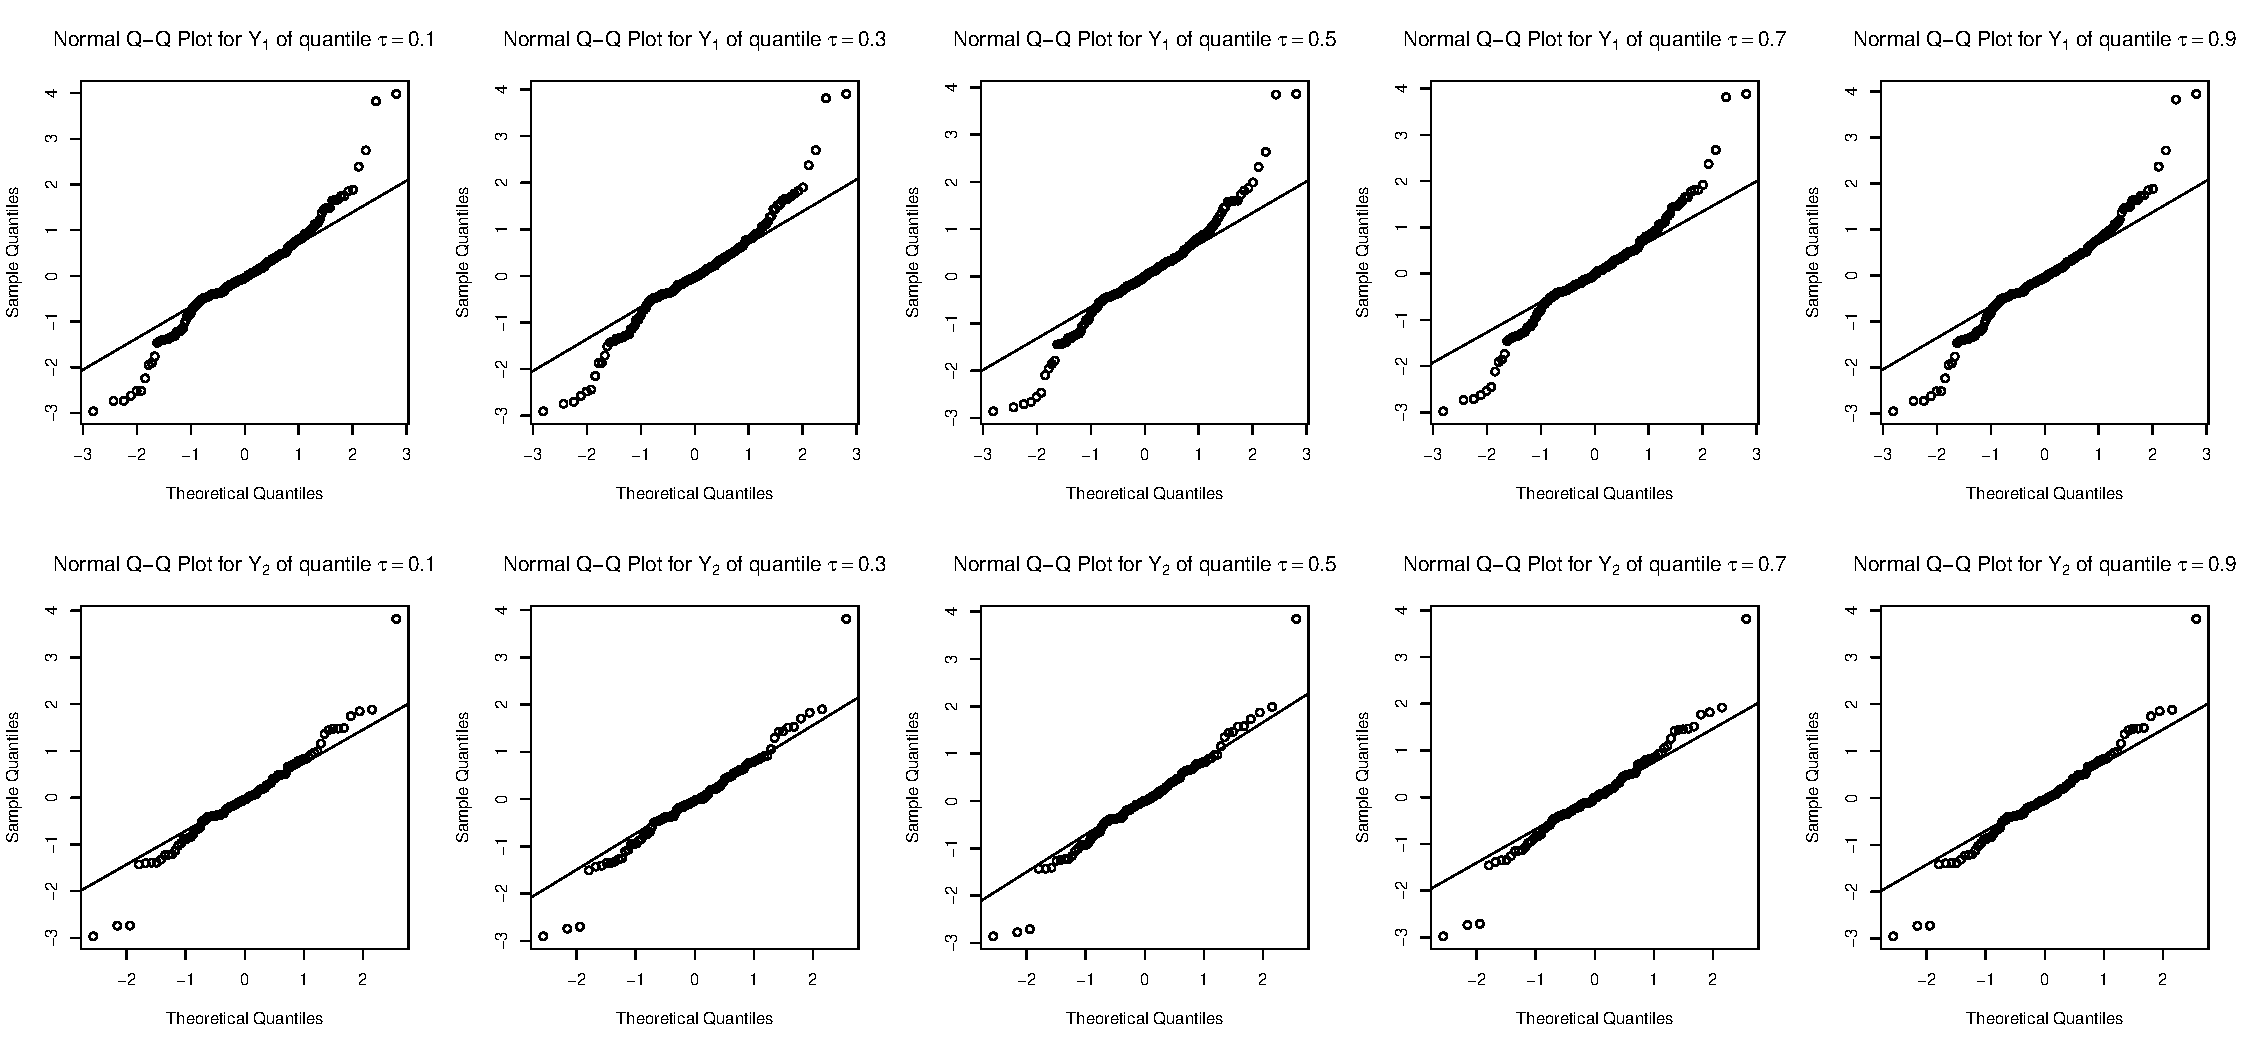
\includegraphics[scale=.4]{../image/T3S3}}
\caption{Goodness of Fit Check for $t_3$ Error under Scenario 3}
\end{figure}

\begin{figure}[h]
\centerline{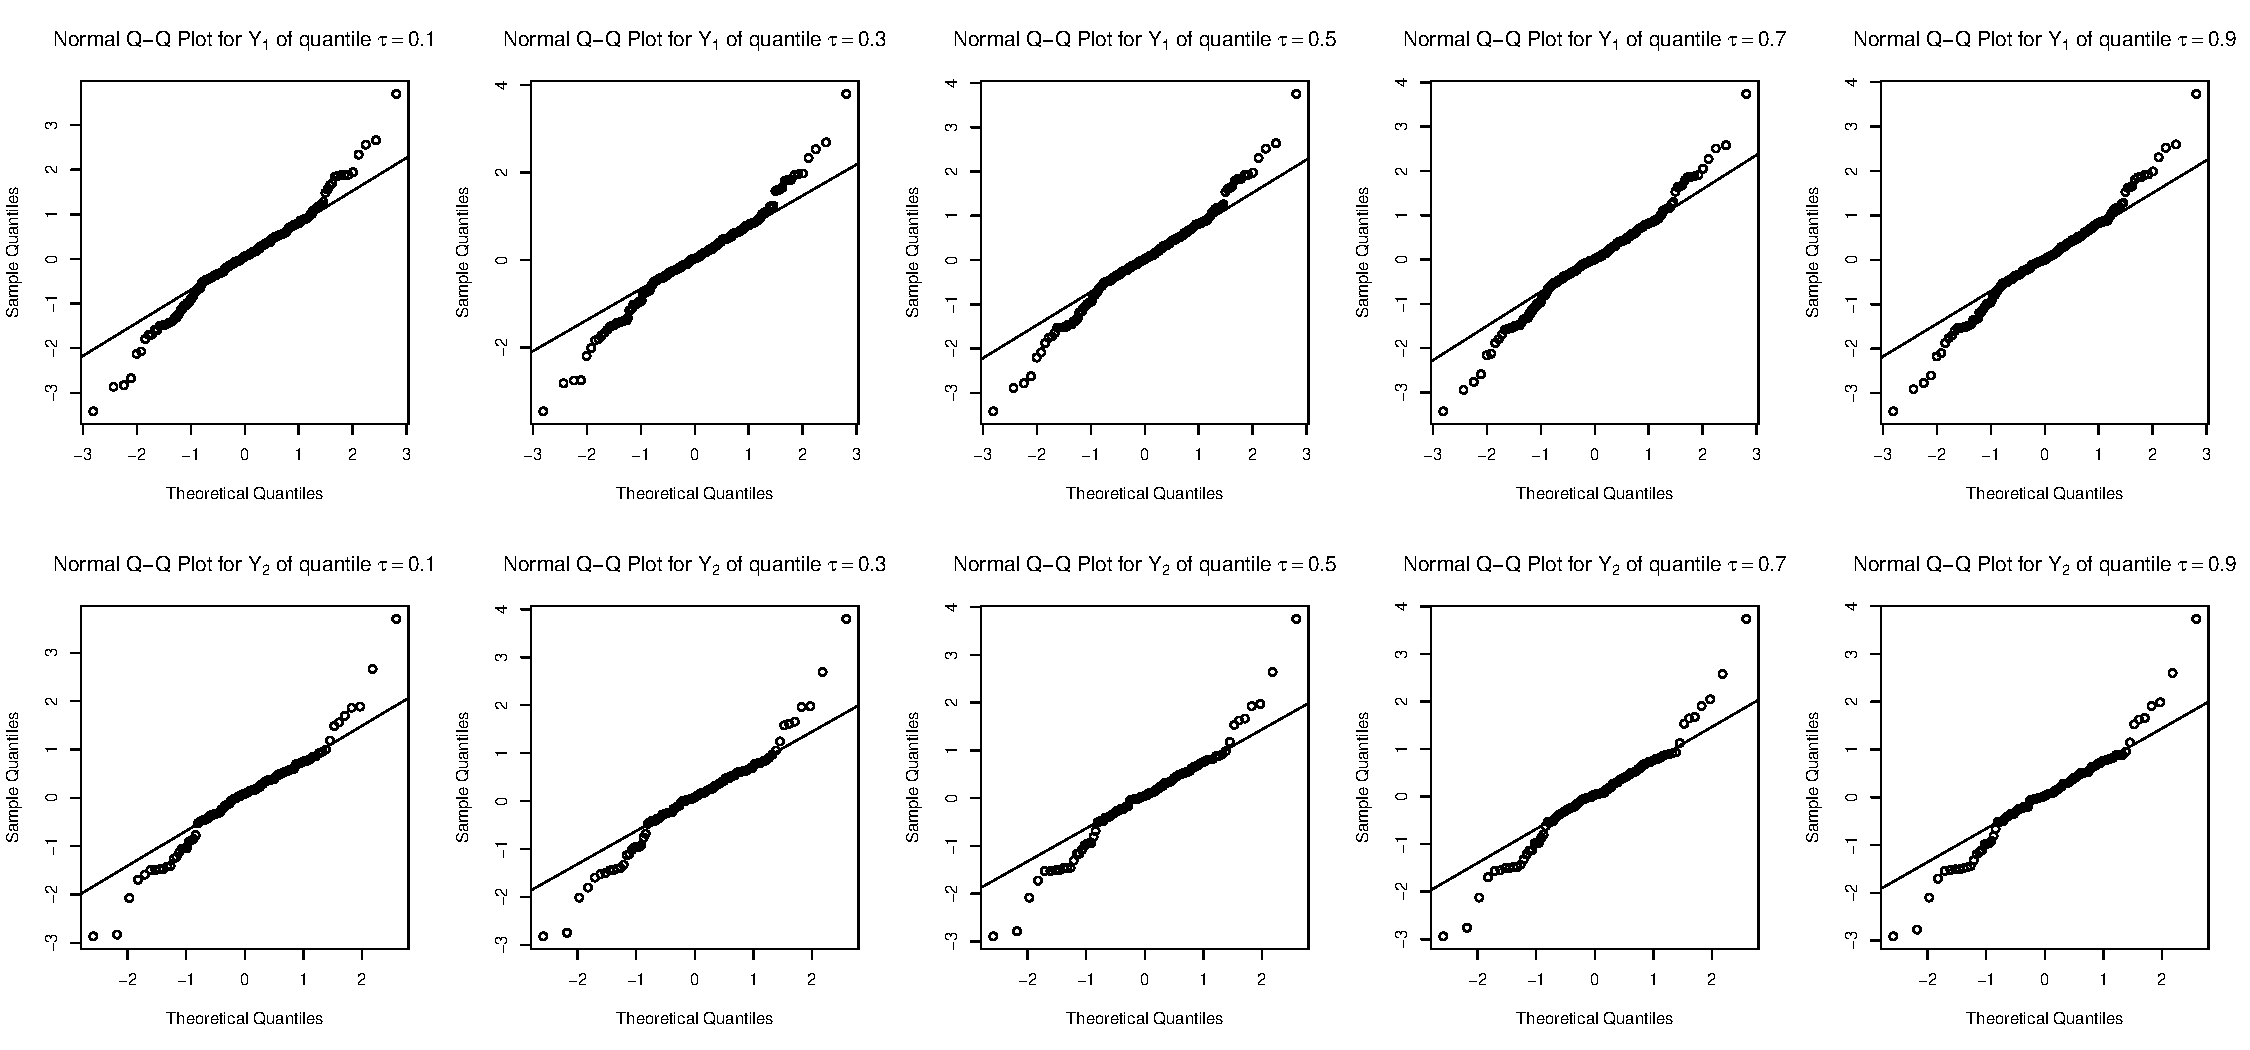
\includegraphics[scale=.4]{../image/LPS1}}
\caption{Goodness of Fit Check for Laplace Error under Scenario 1}
\end{figure}

\begin{figure}[h]
\centerline{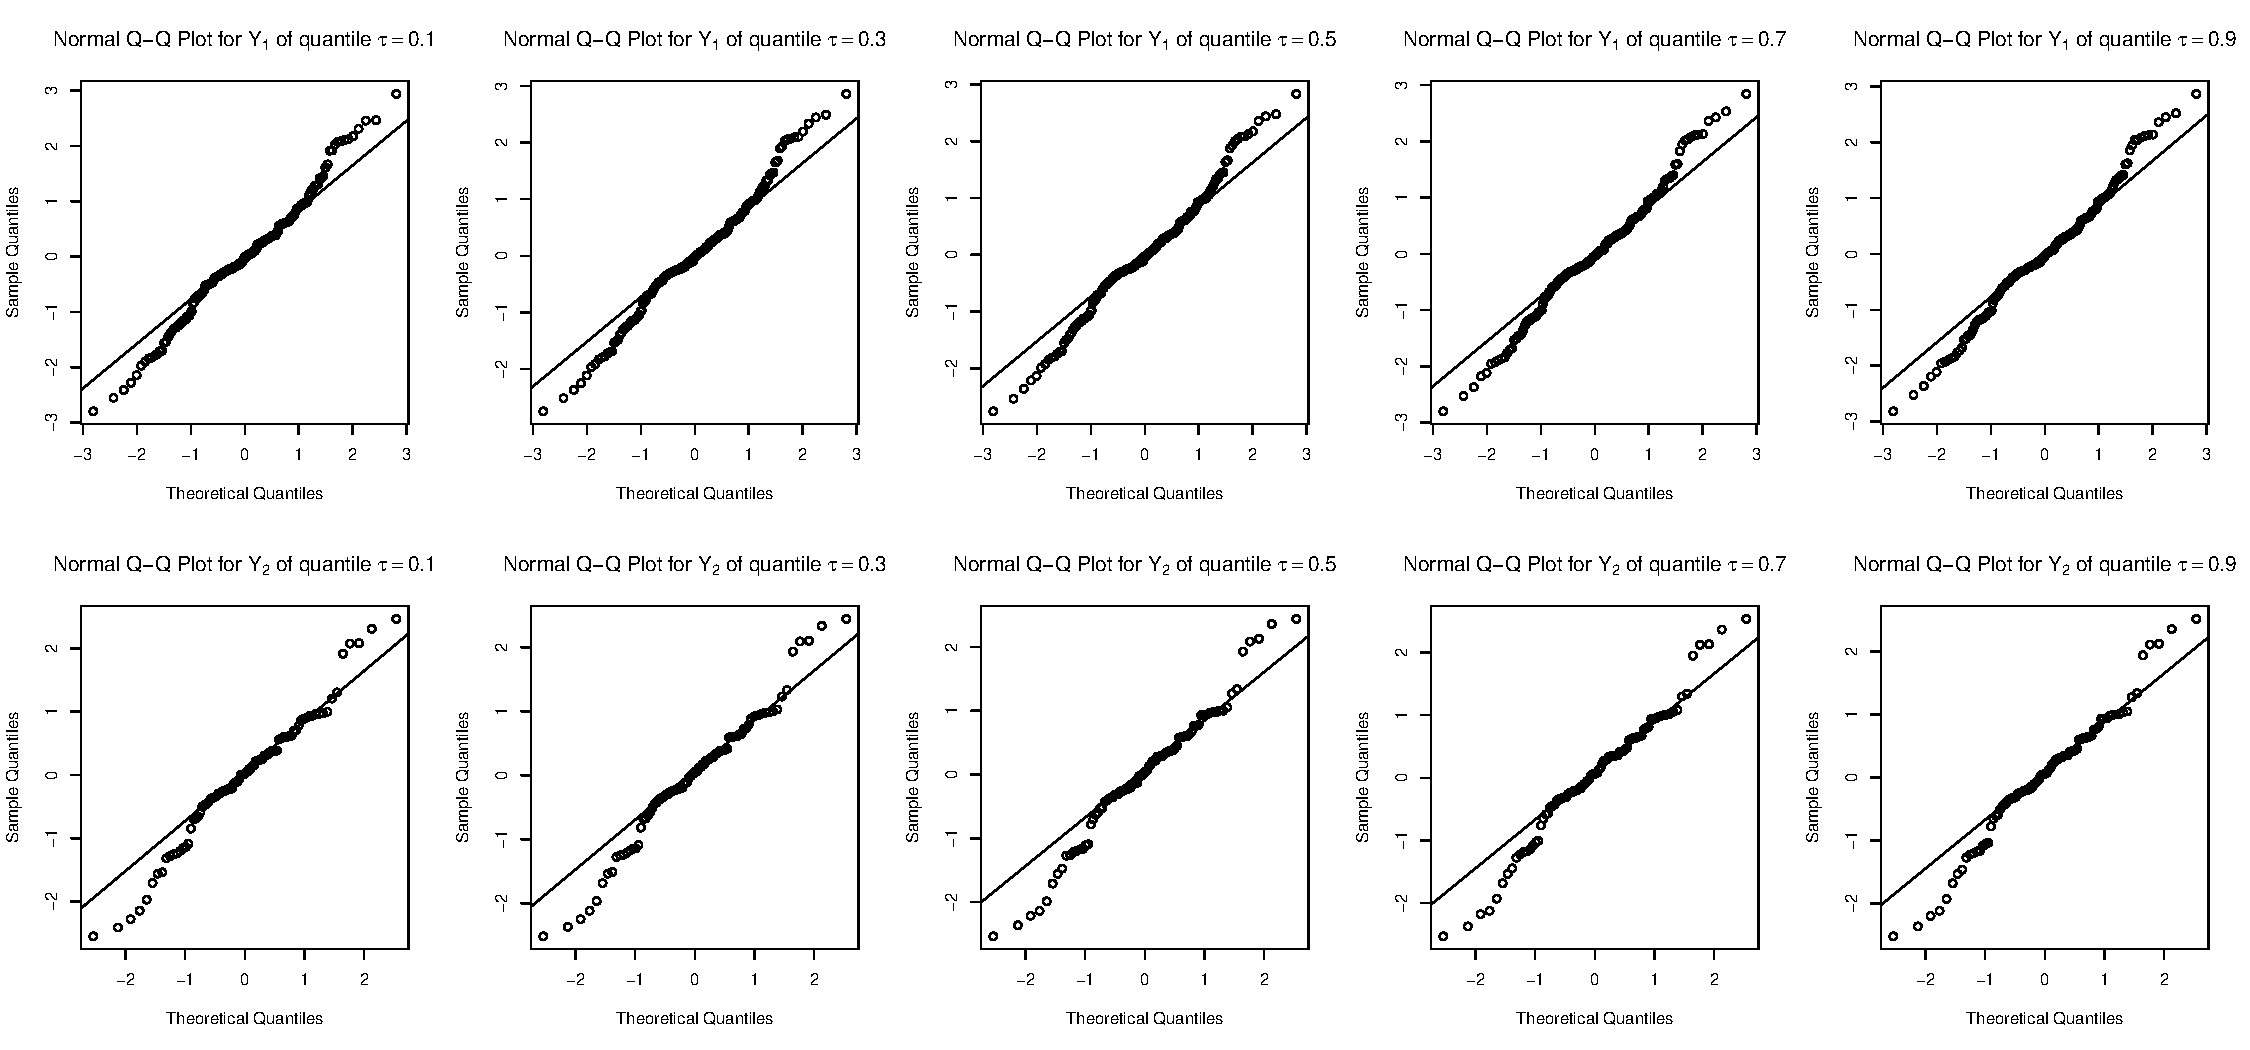
\includegraphics[scale=.4]{../image/LPS2}}
\caption{Goodness of Fit Check for Laplace Error under Scenario 2}
\end{figure}

\begin{figure}[h]
\centerline{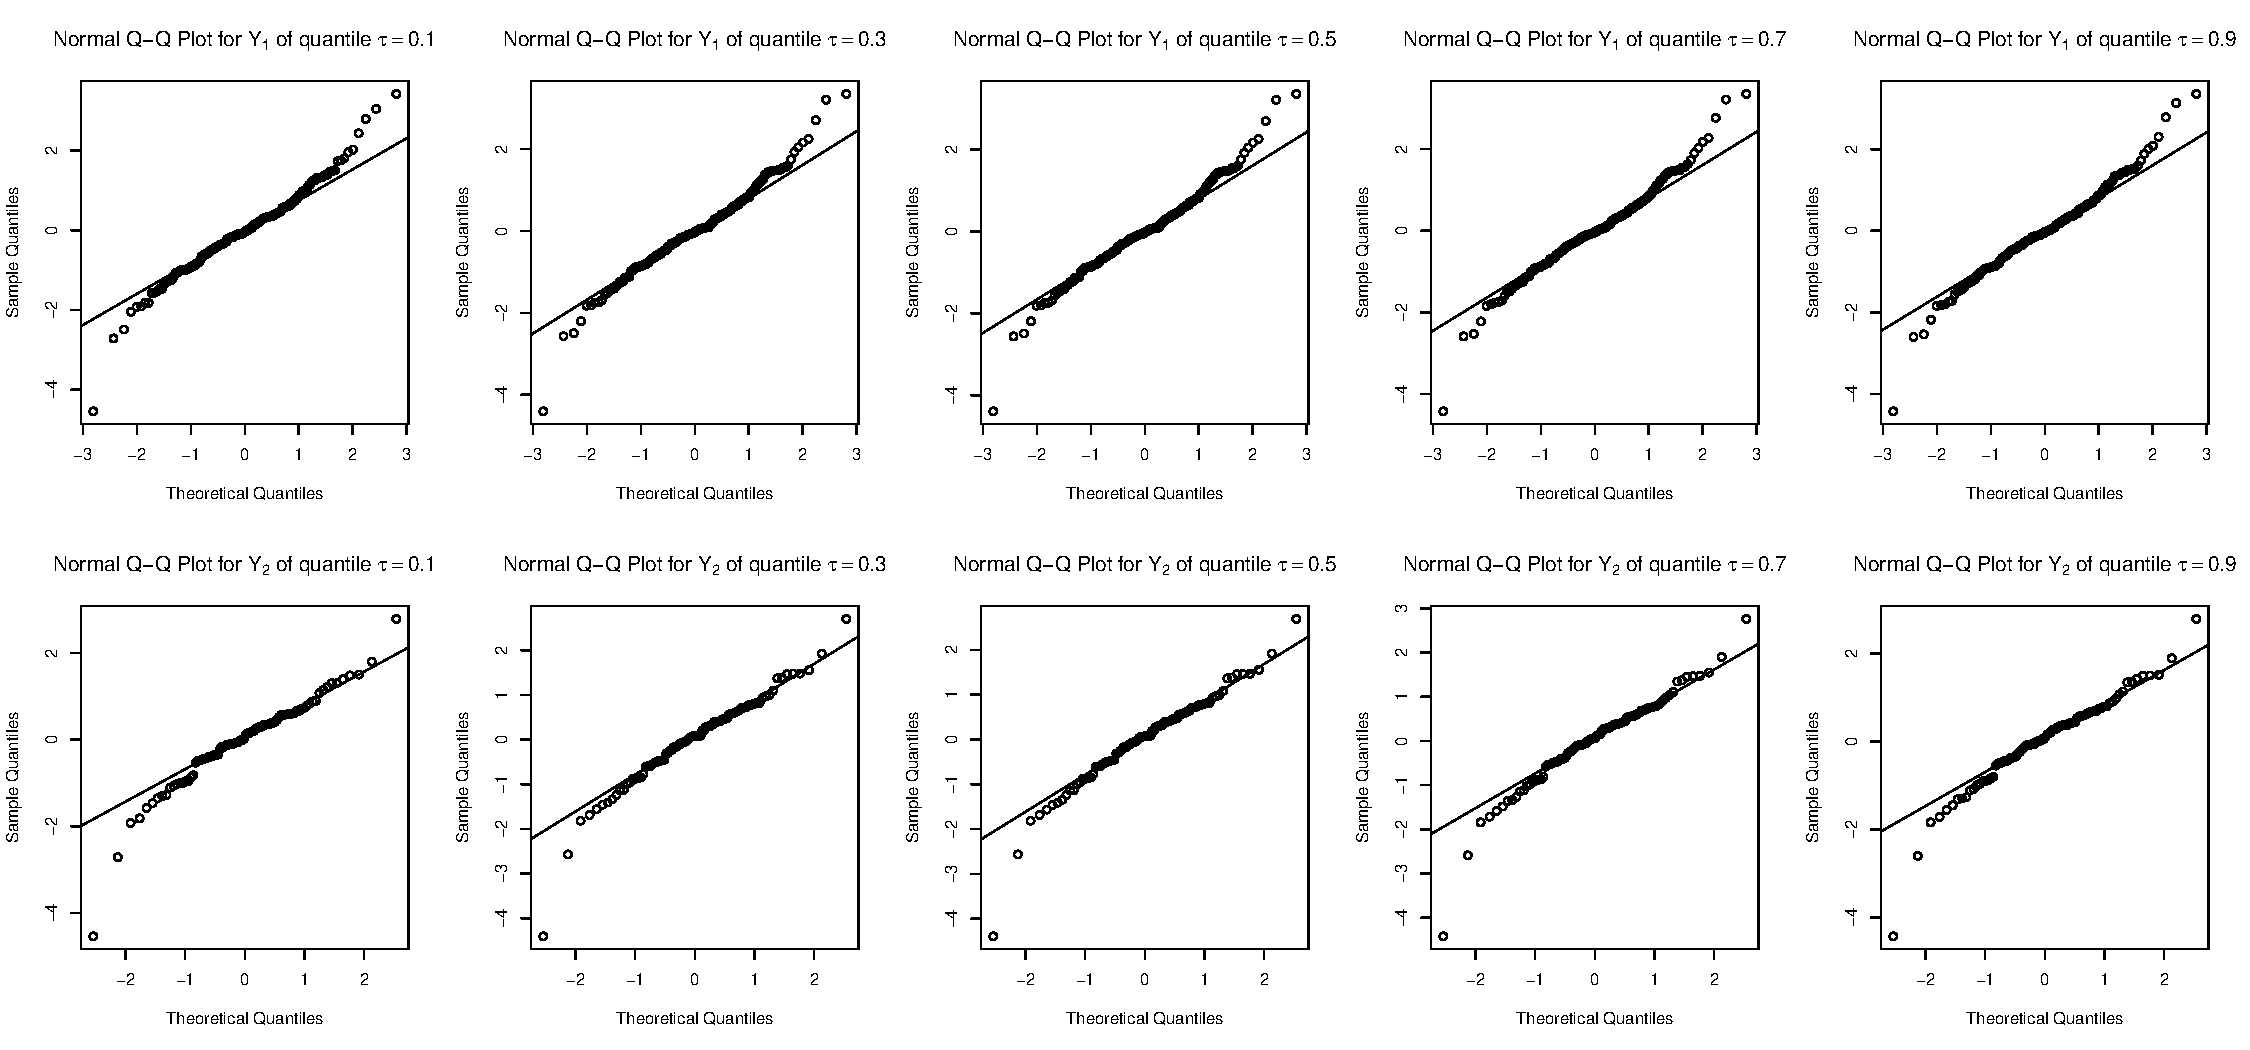
\includegraphics[scale=.4]{../image/LPS3}}
\caption{Goodness of Fit Check for Laplace Error under Scenario 3}
\end{figure}



\end{document}

%%% Local Variables:
%%% mode: latex
%%% End:
